\documentclass{standalone}

\usepackage{graphicx}

\usepackage{microtype}
\usepackage{pgfplots}
\pgfplotsset{compat=1.18}
\usepackage{tikz}
\usetikzlibrary{positioning, arrows.meta, fit, shapes.geometric, calc}


\begin{document}
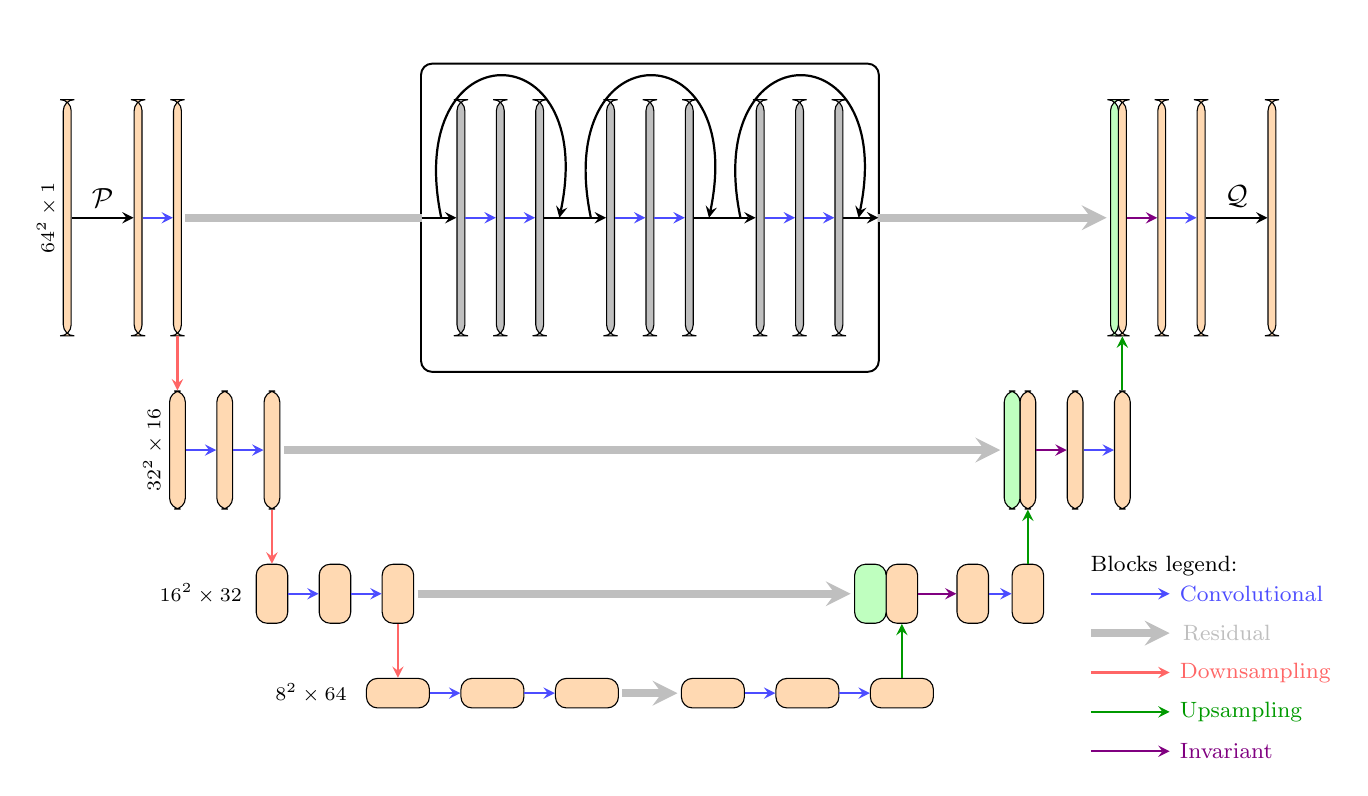
\begin{tikzpicture}[
    % Styles
    scale=1,
    box/.style n args={2}{
            draw,
            rounded corners,
            align=center,
            minimum height=#1,
            minimum width=#2,
            text width=#2,
            inner sep=0pt,
            fill=orange!30
        },
    greenbox/.style n args={2}{
            draw,
            rounded corners,
            align=center,
            minimum height=#1,
            minimum width=#2,
            text width=#2,
            inner sep=0pt,
            fill=green!25
        },
    graybox/.style n args={2}{
            draw,
            rounded corners,
            align=center,
            minimum height=#1,
            minimum width=#2,
            text width=#2,
            inner sep=0pt,
            fill=gray!50
        },
    conv/.style={-stealth, blue!70, thick},
    inv/.style={-stealth, violet, thick},
    connection/.style={-stealth, black, thick},
    pool/.style={-stealth, red!60, thick},
    upconv/.style={-stealth, green!60!black, thick},
    copy/.style={-stealth, gray!50, line width=0.1cm},
    copynoarrow/.style={gray!50, line width=0.1cm},
    label/.style={font=\scriptsize, align=center},
    legend/.style={font=\footnotesize, align=left}
]

% Parameters of boxes
\def\boxwidth{0.1cm}
\def\boxheight{3cm}
\def\scale{0.5}

% parameters of labels
\def\bufflabel{4}

% Spacing between boxes
\def\spacing{0.4cm}
\def\vspacing{0.7cm}

% Buffer for arrow
\def\buffarrow{0.05cm}

% Contracting Path (Encoder)
\node[box={\boxheight}{\boxwidth}] (l1) at (-\spacing,0) {};
\node[label, rotate=90] at (-\boxwidth/2-1.5*\bufflabel-\spacing, 0) {$64^2\times 1$};

\node[box={\boxheight}{\boxwidth}] (l2) at (\boxwidth+\spacing,0) {};

\node[box={\boxheight}{\boxwidth}] (l3) at (2*\boxwidth+2*\spacing,0) {};

\node[box={\boxheight*\scale}{2*\boxwidth}] (l4) at (2*\boxwidth+2*\spacing,-\boxheight/2 -\boxheight*\scale/2-\vspacing) {};
\node[label, rotate=90] at ($(l4)+(-\boxwidth-1.5*\bufflabel, 0)$) {$32^2\times 16$};

\node[box={\boxheight*\scale}{2*\boxwidth}] (l5) at (4*\boxwidth+3*\spacing,-\boxheight/2 -\boxheight*\scale/2-\vspacing) {};

\node[box={\boxheight*\scale}{2*\boxwidth}] (l6) at (6*\boxwidth+4*\spacing,-\boxheight/2 -\boxheight*\scale/2-\vspacing) {};

\node[box={\boxheight*\scale^2}{4*\boxwidth}] (l7) at (6*\boxwidth+4*\spacing, -\boxheight/2 -\boxheight*\scale-\boxheight*\scale^2/2-2*\vspacing) {};
\node[label] at ($(l7)+(-2*\boxwidth-5*\bufflabel, 0)$) {$16^2\times 32$};

\node[box={\boxheight*\scale^2}{4*\boxwidth}] (l8) at (10*\boxwidth+5*\spacing,-\boxheight/2 -\boxheight*\scale-\boxheight*\scale^2/2-2*\vspacing) {};

\node[box={\boxheight*\scale^2}{4*\boxwidth}] (l9) at (14*\boxwidth+6*\spacing,-\boxheight/2 -\boxheight*\scale-\boxheight*\scale^2/2-2*\vspacing) {};

% Bottom Part (Bottleneck)
\node[box={\boxheight*\scale^3}{8*\boxwidth}] (b1) at (14*\boxwidth+6*\spacing,-\boxheight/2 -\boxheight*\scale-\boxheight*\scale^2-\boxheight*\scale^3/2-3*\vspacing) {};
\node[label] at ($(b1)+(-4*\boxwidth-5*\bufflabel, 0)$) {$8^2\times 64$};

\node[box={\boxheight*\scale^3}{8*\boxwidth}] (b2) at (22*\boxwidth+7*\spacing,-\boxheight/2 -\boxheight*\scale-\boxheight*\scale^2-\boxheight*\scale^3/2-3*\vspacing) {};

\node[box={\boxheight*\scale^3}{8*\boxwidth}] (b3) at (30*\boxwidth+8*\spacing,-\boxheight/2 -\boxheight*\scale-\boxheight*\scale^2-\boxheight*\scale^3/2-3*\vspacing) {};

% Expansive Path (Decoder)
\node[box={\boxheight*\scale^3}{8*\boxwidth}] (r1) at (30*\boxwidth+12*\spacing,-\boxheight/2 -\boxheight*\scale-\boxheight*\scale^2-\boxheight*\scale^3/2-3*\vspacing) {};

\node[box={\boxheight*\scale^3}{8*\boxwidth}] (r2) at (38*\boxwidth+13*\spacing,-\boxheight/2 -\boxheight*\scale-\boxheight*\scale^2-\boxheight*\scale^3/2-3*\vspacing) {};

\node[box={\boxheight*\scale^3}{8*\boxwidth}] (r3) at (46*\boxwidth+14*\spacing,-\boxheight/2 -\boxheight*\scale-\boxheight*\scale^2-\boxheight*\scale^3/2-3*\vspacing) {};

\node[box={\boxheight*\scale^2}{4*\boxwidth}] (r4) at (46*\boxwidth+14*\spacing,-\boxheight/2 -\boxheight*\scale-\boxheight*\scale^2/2-2*\vspacing) {};
\node[greenbox={\boxheight*\scale^2}{4*\boxwidth}] (r4-l) at (42*\boxwidth+14*\spacing,-\boxheight/2 -\boxheight*\scale-\boxheight*\scale^2/2-2*\vspacing) {};

\node[box={\boxheight*\scale^2}{4*\boxwidth}] (r5) at (51*\boxwidth+15*\spacing,-\boxheight/2 -\boxheight*\scale-\boxheight*\scale^2/2-2*\vspacing) {};

\node[box={\boxheight*\scale^2}{4*\boxwidth}] (r6) at (54*\boxwidth+16*\spacing,-\boxheight/2 -\boxheight*\scale-\boxheight*\scale^2/2-2*\vspacing) {};

\node[box={\boxheight*\scale}{2*\boxwidth}] (r7) at (54*\boxwidth+16*\spacing,-\boxheight/2 -\boxheight*\scale/2-\vspacing) {};
\node[greenbox={\boxheight*\scale}{2*\boxwidth}] (r7-l) at (52*\boxwidth+16*\spacing,-\boxheight/2 -\boxheight*\scale/2-\vspacing) {};

\node[box={\boxheight*\scale}{2*\boxwidth}] (r8) at (56*\boxwidth+17*\spacing,-\boxheight/2 -\boxheight*\scale/2-\vspacing) {};

\node[box={\boxheight*\scale}{2*\boxwidth}] (r9) at (58*\boxwidth+18*\spacing,-\boxheight/2 -\boxheight*\scale/2-\vspacing) {};

% Residual block example
\node[graybox={\boxheight}{\boxwidth}] (res1) at (26*\boxwidth+5*\spacing,0) {};
\node[graybox={\boxheight}{\boxwidth}] (res2) at (27*\boxwidth+6*\spacing,0) {};
\node[graybox={\boxheight}{\boxwidth}] (res3) at (28*\boxwidth+7*\spacing,0) {};
\node[graybox={\boxheight}{\boxwidth}] (res4) at (29*\boxwidth+9*\spacing,0) {};
\node[graybox={\boxheight}{\boxwidth}] (res5) at (30*\boxwidth+10*\spacing,0) {};
\node[graybox={\boxheight}{\boxwidth}] (res6) at (31*\boxwidth+11*\spacing,0) {};
\node[graybox={\boxheight}{\boxwidth}] (res7) at (32*\boxwidth+13*\spacing,0) {};
\node[graybox={\boxheight}{\boxwidth}] (res8) at (33*\boxwidth+14*\spacing,0) {};
\node[graybox={\boxheight}{\boxwidth}] (res9) at (34*\boxwidth+15*\spacing,0) {};
\node[draw, line width = .7pt, rounded corners, inner sep=0.45cm, fit= (res1) (res2) (res3) (res4) (res5) (res6) (res7) (res8) (res9)] (internal) {};

% Final Output Path
\node[box={\boxheight}{\boxwidth}] (f1) at (58*\boxwidth+18*\spacing,0) {};
\node[greenbox={\boxheight}{\boxwidth}] (f1-l) at (57*\boxwidth+18*\spacing,0) {};

\node[box={\boxheight}{\boxwidth}] (f2) at (59*\boxwidth+19*\spacing,0) {};

\node[box={\boxheight}{\boxwidth}] (f3) at (60*\boxwidth+20*\spacing,0) {};

\node[box={\boxheight}{\boxwidth}] (f4) at (61*\boxwidth+22*\spacing,0) {};

% Connections
% Contracting Path
\draw[connection] (l1) -- (l2) node[midway, above] {$\mathcal{P}$};
\draw[conv] (l2) -- (l3);
\draw[pool] (l3) -- (l4);
\draw[conv] (l4) -- (l5);
\draw[conv] (l5) -- (l6);
\draw[pool] (l6) -- (l7);
\draw[conv] (l7) -- (l8);
\draw[conv] (l8) -- (l9);
\draw[pool] (l9) -- (b1);

% Bottom
\draw[conv] (b1) -- (b2);
\draw[conv] (b2) -- (b3);

% Expansive Path
\draw[conv] (r1) -- (r2);
\draw[conv] (r2) -- (r3);
\draw[upconv] (r3) -- (r4);
\draw[inv] (r4) -- (r5);
\draw[conv] (r5) -- (r6);
\draw[upconv] (r6) -- (r7);
\draw[inv] (r7) -- (r8);
\draw[conv] (r8) -- (r9);
\draw[upconv] (r9) -- (f1);
\draw[inv] (f1) -- (f2);
\draw[conv] (f2) -- (f3);
\draw[connection] (f3) -- (f4) node[midway, above] {$\mathcal{Q}$};

% Copy Connections
\draw[copynoarrow] ($(l3) + (\boxwidth/2+\buffarrow, 0)$) -- ($(res1) - (0.5, 0)$);
\draw[copy] ($(res9) + (0.5, 0)$) -- ($(f1-l) - (\boxwidth/2+\buffarrow, 0)$);
\draw[copy] ($(l6) + (\boxwidth+\buffarrow, 0)$) -- ($(r7-l) - (\boxwidth+\buffarrow, 0)$);
\draw[copy] ($(l9) + (2*\boxwidth+\buffarrow, 0)$) -- ($(r4-l) - (2*\boxwidth+\buffarrow, 0)$);
\draw[copy] ($(b3) + (4*\boxwidth+\buffarrow, 0)$) -- ($(r1) - (4*\boxwidth+\buffarrow, 0)$);

% Residual Connections
\draw[connection] ($(res1) - (0.5, 0)$)-- (res1);
\draw[conv] (res1) -- (res2);
\draw[conv] (res2) -- (res3);
% \draw[connection] ($(res1) + (0, \boxheight/2+1)$) to[out=70, in=110] ($(res3) + (0, \boxheight/2+1)$);
\draw[connection] ($(res1) + (-0.25, 0)$) .. controls +(-0.5,2.4) and +(0.5,2.4) .. ($(res3) + (0.25, 0)$);
\draw[connection] (res3) -- (res4);
\draw[conv] (res4) -- (res5);
\draw[conv] (res5) -- (res6);
% \draw[connection] ($(res4) + (0, \boxheight/2+1)$) to[out=70, in=110] ($(res6) + (0, \boxheight/2+1)$);
\draw[connection] ($(res4) + (-0.25, 0)$) .. controls +(-0.5,2.4) and +(0.5,2.4) .. ($(res6) + (0.25, 0)$);
\draw[connection] (res6) -- (res7);
\draw[conv] (res7) -- (res8);
\draw[conv] (res8) -- (res9);
% \draw[connection] ($(res7) + (0, \boxheight/2+1)$) to[out=70, in=110] ($(res9) + (0, \boxheight/2+1)$);
\draw[connection] ($(res7) + (-0.25, 0)$) .. controls +(-0.5,2.4) and +(0.5,2.4) .. ($(res9) + (0.25, 0)$);
\draw[connection] (res9) -- ($(res9) + (0.5, 0)$);

% Legend
\begin{scope}[shift={(58*\boxwidth+17*\spacing,-\boxheight/2 -\boxheight*\scale-\boxheight*\scale^2/2-2*\vspacing)}]
    \draw[conv] (0,0) -- (1,0) node[legend, right] {Convolutional} node[legend, black, yshift=10, xshift=-2] {Blocks legend:};
    \draw[copy] (0,-0.5) -- (1,-0.5) node[legend, right] {Residual};
    \draw[pool] (0,-1) -- (1,-1) node[legend, right] {Downsampling};
    \draw[upconv] (0,-1.5) -- (1,-1.5) node[legend, right] {Upsampling};
    \draw[inv] (0,-2) -- (1,-2) node[legend, right] {Invariant};
\end{scope}
\end{tikzpicture}
\end{document}